\chapter{Results} \label{chap_4}
\ \\
To correctly analyze and categorize the bugs discovered you need to perform \textit{bug deduplication}, a technique used to remove all inputs that produced the same results, which is crucial to remove unnecessary data from the results and make the bug analysis work less tedious for the developer. There are several strategies that can be applied to deduplicate bugs, but it's important to mention that there is no fool-proof methodology that produces perfect results on all possible scenarios, and this is because which information you are using as reference and their number will (almost always) lead to partial loss of data.

Given that this work focused primarily on frameworks based on ClusterFuzz as the back-end, I decided to employ the same approach used by ClusterFuzz when generating bug reports, where the fields "Crash Type" and "Crash state" are the main references (recall figure \ref{fig:issue}). To do this, I used several Python scripts (one for each sanitizer and one for Valgrind) that analyzed the logs generated during each fuzzing sessions, and deduplication was performed by its \textit{"error type"} and the last 3 stack entries from where the error occurred.

Then, \textit{bug triage} was performed, analyzing more in depth where the bug occurred, why it happened and assigning a priority in the range "Low", "Medium" and "High". This required a manual investigation of each bug individually, statically and dynamically (when available), to have a more clear understanding of the problem and potentially provide suggestions to the developers regarding the fix.
This step was also important to refine the previous deduplication step.  Assume the situation where two inputs triggered two (apparently) different bugs because they have distinct stack flows: if the bug originated from the same function, it meant that two different execution flows triggered the same error. In this case, a common practice is to fix one of them and then use the other input as an additional check for correctness.

Finally, all recorded bugs for a project, along with their log and fuzz targets, were reported to their respective developers.
At the moment of writing, unfortunately, not all developers answered and/or acknowledged the reported bugs.




\section{OSS-Fuzz (aggiornare la tabella fino all'ultimo!)}
\begin{adjustbox}{width=\textwidth,center}
\begin{tabular}{|l|l|l|l|l|l|l|l|l|}
\hline
\textbf{Project} & \textbf{Sanitizers} & \textbf{Queue size} & \textbf{Crashes} & \textbf{ASan} & \textbf{Valgrind} & \textbf{UBSan} & \textbf{Total} & \textbf{Confirmed}  \\ 
\hline
binutils         & ALL                 & $20,274$            & $0$              & $0$           & $1$           & $0$            & $1$             & $1$                 \\
harfbuzz         & ALL                 & $23,357$            & $0$              & $0$           & $1$           & $0$            & $1$             & $1$                 \\
imagemagick      & ALL                 & $9,470$             & $0$              & $0$           & $6$           & $1$            & $7$             & $1$                 \\
libxml2          & ALL                 & $13,474$            & $0$              & $0$           & $0$           & $0$            & $0$             & $0$                 \\
skia             & ALL                 & $18,295$            & $0$              & $0$           & $0$           & $0$            & $0$             & $0$                 \\ 
\hline
ghostscript      & A+M                 & $9,917$             & $0$              & $0$           & $32$          & $1$            & $33$            & $33$                \\
libyang          & A+M                 & $8,745$             & $0$              & $0$           & $0$           & $0$            & $0$             & $0$                 \\
myanmar-tools    & A+M                 & $448$               & $0$              & $0$           & $0$           & $0$            & $0$             & $0$                 \\
openjpeg         & A+M                 & $8,856$             & $0$              & $0$           & $0$           & $0$            & $0$             & $0$                 \\
wasmedge         & A+M                 & $9,454$             & $0$              & $0$           & $0$           & $0$            & $0$             & $0$                 \\ 
\hline
cairo            & A+UB                & $15,870$            & $0$              & $1$           & $1$           & $28$           & $30$            & $0$                 \\
clamav           & A+UB                & $6,742$             & $0$              & $0$           & $0$           & $2$            & $2$             & $0$                 \\
freerdp          & A+UB                & $7,607$             & $0$              & $0$           & $0$           & $1$            & $1$             & $1$                 \\
tarantool        & A+UB                & $10,987$            & $0$              & $0$           & $1$           & $0$            & $1$             & $1$                 \\
vlc              & A+UB                & $16,018$            & $2$              & $1$           & $2$           & $4$            & $9$             & $5$                 \\ 
\hline
fwupd            & ASan only                & $5,843$             & $0$              & $0$           & $0$           & $0$            & $0$             & $0$                 \\
glslang          & ASan only                & $14,534$            & $0$              & $1$           & $1$           & $0$            & $1$             & $1$                 \\
inchi            & ASan only                & $12,034$            & $0$              & $1$           & $4$           & $3$            & $8$             & $8$                 \\
radare2          & ASan only                & $9,914$             & $0$              & $1$           & $0$           & $9$            & $10$            & $10$                \\
zeek             & ASan only                & $8,390$             & $0$              & $0$           & $1$           & $5$            & $6$             & $6$                 \\ 
\hline
fluent-bit       & NONE                & $4,968$             & $0$              & $0$           & $1$           & $1$            & $2$             & $2$                 \\
gpac             & NONE                & $22,917$            & $2$         & $0$           & $25$          & $0$            & $27$            & $27$                \\
libdwarf         & NONE                & $7,667$             & $0$              & $0$           & $0$           & $0$            & $0$             & $0$                 \\
libredwg         & NONE                & $46,160$            & $0$              & $1$           & $3$           & $0$            & $4$             & $4$                 \\
serenity         & NONE                & $9,940$             & $0$              & $0$           & $1$           & $1$            & $2$             & $2$                 \\
\hline
TOTAL BUGS   &   &   &$4$   &$6$   &$80$   &$56$   &$145$   &$103$       \\
\hline
\end{tabular}
\end{adjustbox}{}
\ \\ 

The above table shows the aggregated results for OSS-Fuzz.

First and foremost, developers have different approaches to bug reporting. The OSS-Fuzz reports were submitted during September, and there are still just under 1/3 of the discovered bugs that have yet to be acknowledged by their respective developers. Although most of them were related to use-of-uninitialized-memory and undefined behaviors, they would require little to none effort to solve them, which shows how many open-source developers either do not have enough time and resources to fix them, or they simply do not care about reports on trivial bugs that are not security relevant and postpone them (sometimes indefinitely).

Then, we can see the effects of using sanitizers during tests. While the projects that were being tested using all sanitizers produced only a total of 9 bugs, the remaining 136 were evenly distributed across the remaining categories: this is a good example of how a sanitizer is beneficial to your program but is not a replacement for programs written following good coding practices. "Ghostscript" uses MSan, yet it has the highest number of memory-related bugs. "Cairo" uses UBSan, yet it has the highest number of undefined-behavior bugs.

We can also infer the popularity of each sanitizer. ASan is the most popular and widely used, reflected by the number of bugs found. UBSan is also among the most used ones, although the statistic shown here is biased by "Cairo": while this project is affected by many UB bugs, specifically improper conversion of data between different types, almost all previous reports on the issue tracker related to similar problems were simply marked as "Wont Fix". Finally, Valgrind's memory analysis yielded the highest number, highlighting how MSan was often not used due to its reports containing too many false positives.

The reasons why this work discovered so many bugs are up for debate, as the inner workings of such infrastructures are not publicly available most likely due to security reasons, but there are some key hypothesis that can be mentioned.

A trivial explanation lies in the developers' choices when it comes to selecting which sanitizers and fuzzing engines will be used for the tests. Regarding the sanitizers, one would expect to find many bugs of a certain type when introducing a sanitizer that is not already being used by OSS-Fuzz. Moreover, each sanitizer generates different types of testcases that may produce new coverage when testing the program with another sanitizer. Also fuzzing engines, similarly to sanitizers, use different approaches and strategies when testing a program: given that each fuzzer generates different new testcases and produces different coverage, using the same corpus with different fuzzers may produce substantially different results. Moreover, although not shown in the previous table, less than half of the projects tested included AFL as one of its fuzzing engines used for the tests: it's interesting to mention that all the projects that used AFL yielded (on average) less bugs that the others, which again highlights why it is considered the current state-of-the-art.

Another reason may lie in the algorithms used by ClusterFuzz to manage the fuzzing queues. Each time a project undergoes a fuzzing session, it will produce a set containing all the interesting input discovered (i.e. produced new coverage) along with any new testcases generated by the fuzzer, that is then manipulated and processed to form what will be the the corpus used as input for future fuzzing sessions. Among the many operations performed, \textit{bug deduplication} and \textit{pruning} are essential to make sure that the size of this corpus does not explode over time. We already established how ClusterFuzz performs \textit{deduplication}, specifically "error type" and the last 3 stack entries, and also mentioned that there is no general solution to this process that does not involve some degree of information loss.
The same can be said about \textit{pruning}, which is the process of removing all unnecessary and non-relevant inputs from a corpus. ClusterFuzz employ several \textit{"Multi-Armed Bandit (MAB)"} \cite{mab} algorithms, whose statistical explanation will be omitted for the sake of simplicity, in the following way: at the end of each fuzzing session, ClusterFuzz must decide whether to prioritize inputs that caused bugs or inputs that produced new coverage, using regress knowledge and implementation choices as reference. Given that ClusterFuzz's developers prioritize code coverage, most inputs from a fuzzing queue will contain that type of inputs, implying that pruning will most likely remove some inputs causing bugs from future fuzzing queues.

Related to the problem of pruning, there is also the versioning problem.
Let's assume that it exists a specific input on the current version of the program that causes a bug. Then, the developers release a new version introducing some changes, including a fix for said bug, and the input is automatically tested (successfully) and removed by ClusterFuzz as it is not relevant anymore. Patching a single input does not necessarily mean that particular type of error has been permanently is fixed: given that the input has been removed from the queue, unless another input on future fuzzing queues reproduces the problem, it persists. This is the reason why keeping old inputs that caused bugs and testing old corpora on newer versions is useful, as it is not uncommon for developers to reintroduce old bugs during changes, and they might produce interesting and unexpected results.

Finally, we mention how ClusterFuzz handles bugs that cannot be reliably reproduced \cite{unreliable}: 
\textit{"ClusterFuzz does not consider testcases that do not reliably reproduce as important. However, if a crash state is seen very frequently despite not having a single reliable testcase for it, ClusterFuzz will file a bug for it. When ClusterFuzz finds a reliably reproducible testcase for the same crash state, it creates a new report and deletes the older report with the unreliable testcase."}
During this analysis, there were few inputs that did not produce a bug consistently (i.e. the bug did not appear on all execution with the same testcase as input), something that was obviously mentioned in the reports containing them. Given that it is unknown how many times a crash must be "seen" by ClusterFuzz before a generic bug report for it is produced, it's possible that the reports generated during this work may be related to bugs already known by ClusterFuzz but that were not appearing enough times to be considered relevant.


\newpage
\subsection{Case study: GPAC}
The \textit{"GPAC Project on Advanced Content"} (abbreviated \textit{GPAC)} \cite{gpac} is a free and open-source multimedia framework that provides tools to process, inspect, package, stream, media playback and interact with media content, making it a popular choice also among major broadcasters such as Netflix.

Its analysis yielded a total of 27 bugs, 2 crashes and 25 memory-related bugs.
The crashes were related to a SEGV signal sent as a consequence of the process attempting to access address \verb|0x0| (i.e. zero page), which is the first page of a computer's memory and whose access is prohibited and causes an access violation fault, shown below:
\begin{figure}[h]
\makebox[\textwidth][c]{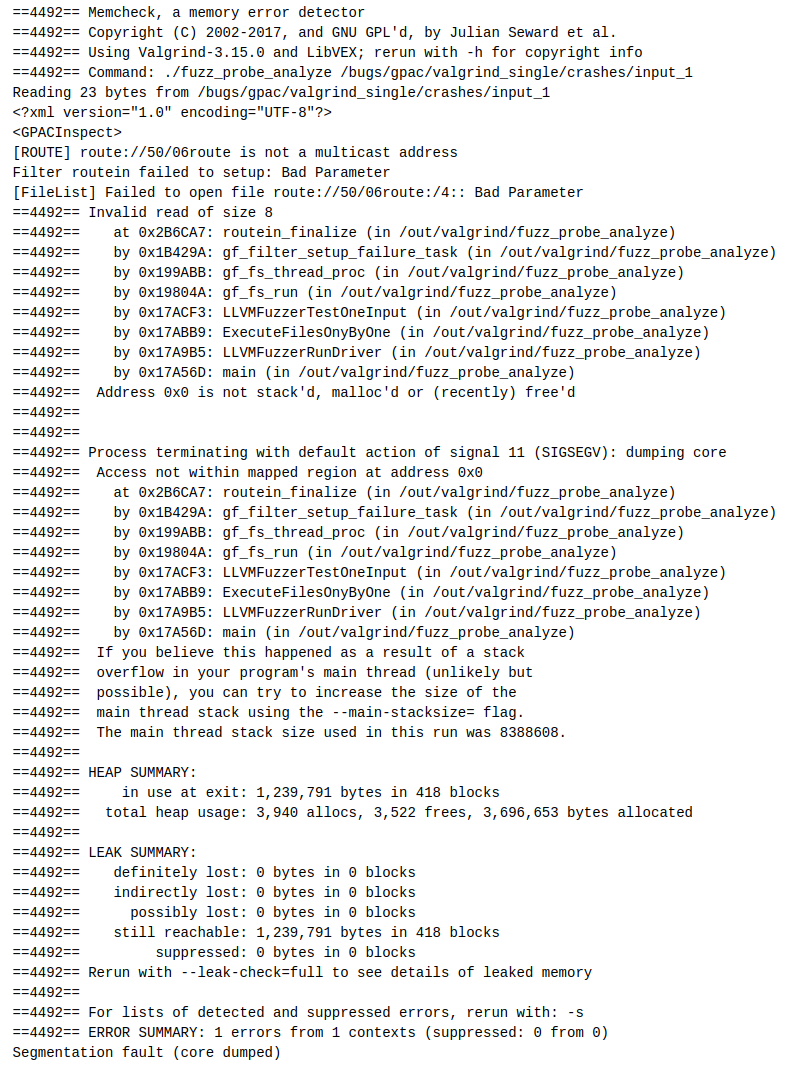
\includegraphics[width=0.55\paperwidth]{foto/segv_gpac.png}}
\caption{Memory access violation reported by Valgrind \ziosaba{Worth it? Remove image?}}
\label{fig:segv_gpac}
\end{figure}
\ \\
It's interesting to note that these bugs have already been reported by ClusterFuzz when discovered by this work and, more importantly, they were still in the bug disclosure windows: this meant that the inputs causing these bugs were not meant to be added to later fuzzing queues and should have not be publicly accessible and available, due to obvious security implications.

This highlights a severe lack of monitoring from both OSS-Fuzz maintainers and the project's developers when it comes to making sure that crucial vulnerabilities are kept private, as indicated by the bug disclosure guidelines.

\ziosaba{I'm not exactly sure what else is there to say about the crashes. Blame it on the human? Blame it on the machine? Also, is it correct what I've written? Not really sure}
The remaining 25 memory bugs were mostly related to use-of-uninitialized-memory (UUM) and memory-bound errors, more specifically:
\begin{itemize}
    \item \textit{conditional jump or move depends on uninitialized value}
    \item \textit{use of uninitialized value in function [...]}
    \item \textit{invalid read of size [...]}
\end{itemize}
The first error happens when an \verb|if| statement is based on a variable whose value is uninitialized.

The second error happens when one (or more) of the parameters passed to an invoked function are uninitialized.

The third error happens when a read/write operation performed overruns the provided buffer, as the content outside of a buffer could be anything.

All these errors, albeit easy to spot and fix, may lead to undefined behavior.
After reporting the UUM bugs and having the pleasure of interacting with the CEO of GPAC itself, we were happy to discover all bugs fixed in just few days.

Also the developers were grateful for this contribution, as they have recently been battling with seemingly-random bugs causing disruptions with the normal functionality of the program, therefore the report has been valuable in helping them to remove uninitialized variables that were leading to undefined behavior.
\ziosaba{This project was a clear example of something? What else?}

\ziosaba{Also, I would honestly move these "Case Study" subsections in another dedicated section, just because if I have to also make a brief point about how the developers handled the problem and their response, then maybe is better to put them after "Developers' responses" and before "Discussion", so that I can also make cross-reference with what was written before}

\newpage
\subsection{Case study: VLC}
The \textit{VLC Media Player} (commonly known as \textit{VLC}) \cite{vlc} is a free and open-source media player software and streaming media server developed by the "VideoLAN Project", supporting many audio and video compression methods, file formats and providing many free decoding and encoding libraries.

Its analysis yielded a total of 9 bugs spread across all categories: 2 crashes, 1 heap-buffer overflow, 2 memory-related bugs and 4 undefined-behaviors.
The heap-buffer overflow bug was initially presented as an ASan bug related to an invocation of \verb|memcpy| that was copying a structure into another one of the same type, which initially left the developers a bit perplexed. After a further analysis, they discovered that the input provided was triggering some strange behavior in another function of their program, whose output lead to incorrect usage of the copy function and therefore the buffer overflow.
The crashes were both related to a SEGV signal sent as a consequence of the process attempting to access a low address that was not mapped within the process's memory region, causing an access violation fault. After a further analysis, it was later discovered that both problem originated from a series of read/write operations performed on uninitialized values causing undefined behavior, ultimately leading to the process accessing an erroneous address.
The first memory bug was related to a memory-bound error caused by several reads operation overrunning the provided buffers, leading to undefined behavior. At the moment of writing, the problem has yet to be fixed because the developers are discussing whether to rewrite or remove the source file causing the problem, as they argue that it is very insecure and could pose a threat to the overall security of the product.
The second memory bugs was related to a use-of-uninitialized-memory (UUM) bug when opening a provided input media file. At the moment of writing, a fix has been proposed but it has yet to be merged with the main code.
Finally, the undefined-behavior (UB) bugs were all related to signed integer-overflow errors, which are relatively easy to fix.
Yet, at the moment of writing they have not been acknowledged by the developers.
This project was a clear example of the most common behavior encountered during this work when interacting with open-source developers.

When presented with bugs that could potentially lead to vulnerabilities or problems in the normal functionalities of their program, their response is usually quick and the problem is fixed in a short amount of time. 

Instead, when the problems have low or negligible priority (like the undefined-behavior bugs), they either ignore the reports or acknowledge their existence and postpone them indefinitely. 

\ \\ 
 

\matteo{Make a new subsection and talk about what can we learn about this, and how can this issue be fixed by Google.}
\ziosaba{Why not moving this topic in the "Discussion" section?}



\newpage
\section{FuzzBench (aggiornare la tabella fino all'ultimo!)}

\matteo{Kind of the same we did for OSS-Fuzz, let's wait for some data before drafting something, I guess.}

\matteo{We can distinguish between "regular" fuzzbench and sbft? Let's see what the numbres say.}

\subsection{Case study: ???}

\newpage
\section{Developers' responses}
Discuss the reports and the developers' answers, including some considerations about their responses...

\newpage
\section{Discussion}
Discuss the overall results, what was expected and what was unexpected...
Discuss the importance of such results, what can be inferred...
Talk about what could/should be done to improve the situation...
